\documentclass[11pt]{report}

\usepackage[polish]{babel}
\usepackage{csquotes}
\DeclareQuoteAlias[]{dutch}{polish}
\usepackage{polski}
\usepackage{geometry}
\usepackage{listings}
\usepackage{xurl}
\usepackage{hyperref}
\usepackage{import}
\usepackage{multirow}
\usepackage{titling}
\usepackage{anyfontsize}
\usepackage[htt]{hyphenat}
\usepackage{xcolor}
\usepackage{graphicx}
\graphicspath{ {./EiWD_zadanie_04_wykresy/} }
\usepackage{subcaption}
\usepackage[
    style=numeric,
    sorting=nty,
    isbn=false,
    backend=biber, %biber EiWD_zadanie_03
]{biblatex}
\addbibresource{EiWD_zadanie_04.bib}

\newcommand{\prowadzacy}{prof. dr hab. inż. Vasyl Martsenyuk}
\newcommand{\temat}{Użycie \texttt{KNIME} w celu wizualizacji}
\newcommand{\wariant}{1}
\newcommand{\kierunek}{Informatyka}
\newcommand{\stopien}{II}
\newcommand{\tryb}{niestacjonarne}
\newcommand{\semestr}{III}
\newcommand{\grupa}{1}
\newcommand{\nrLab}{4}
\newcommand{\repozytorium}{}

\definecolor{codegreen}{rgb}{0,0.6,0}
\definecolor{codegray}{rgb}{0.5,0.5,0.5}
\definecolor{codepurple}{rgb}{0.58,0,0.82}
\definecolor{backcolour}{rgb}{0.95,0.95,0.92}

\lstdefinestyle{mystyle}{
    backgroundcolor=\color{backcolour},   
    commentstyle=\color{codegreen},
    keywordstyle=\color{magenta},
    numberstyle=\tiny\color{codegray},
    stringstyle=\color{codepurple},
    basicstyle=\ttfamily\footnotesize,
    breakatwhitespace=false,         
    breaklines=true,                 
    captionpos=b,                    
    keepspaces=true,                 
    numbers=left,                    
    numbersep=5pt,                  
    showspaces=false,                
    showstringspaces=false,
    showtabs=false,                  
    tabsize=2
}

\lstset{style=mystyle}

\makeatletter
\renewcommand{\@makechapterhead}[1]{%
\vspace*{0 pt}%
{\setlength{\parindent}{0pt} \raggedright \normalfont
\bfseries\Huge\thechapter.\ #1
\par\nobreak\vspace{40 pt}}}
\makeatother

\newcounter{zadanie}
\newcommand{\zadanie}[1]{
    \refstepcounter{zadanie}
    \filbreak\vspace*{1cm}
    {\noindent\raggedright\Large \textbf{Zadanie~\thezadanie. #1}}
    \vspace{10 pt}\nopagebreak[1]
}

\begin{document}

\title{Eksploracja i wizualizacja danych}
\author{Piotr Rybka}
\date{24.11.2021}

\import{}{EiWD_title_page.tex}

\chapter*{Polecenie}

Na podstawie danych ze zbioru \cite{daneMedyczne} wypróbować podstawowe metody biblioteki \enquote{pyspark}.

\zadanie{Pograć program \enquote{Knime} ze strony \url{https://www.knime.com/downloads} i zainstalować}

\begin{figure}[h]
    \centering
    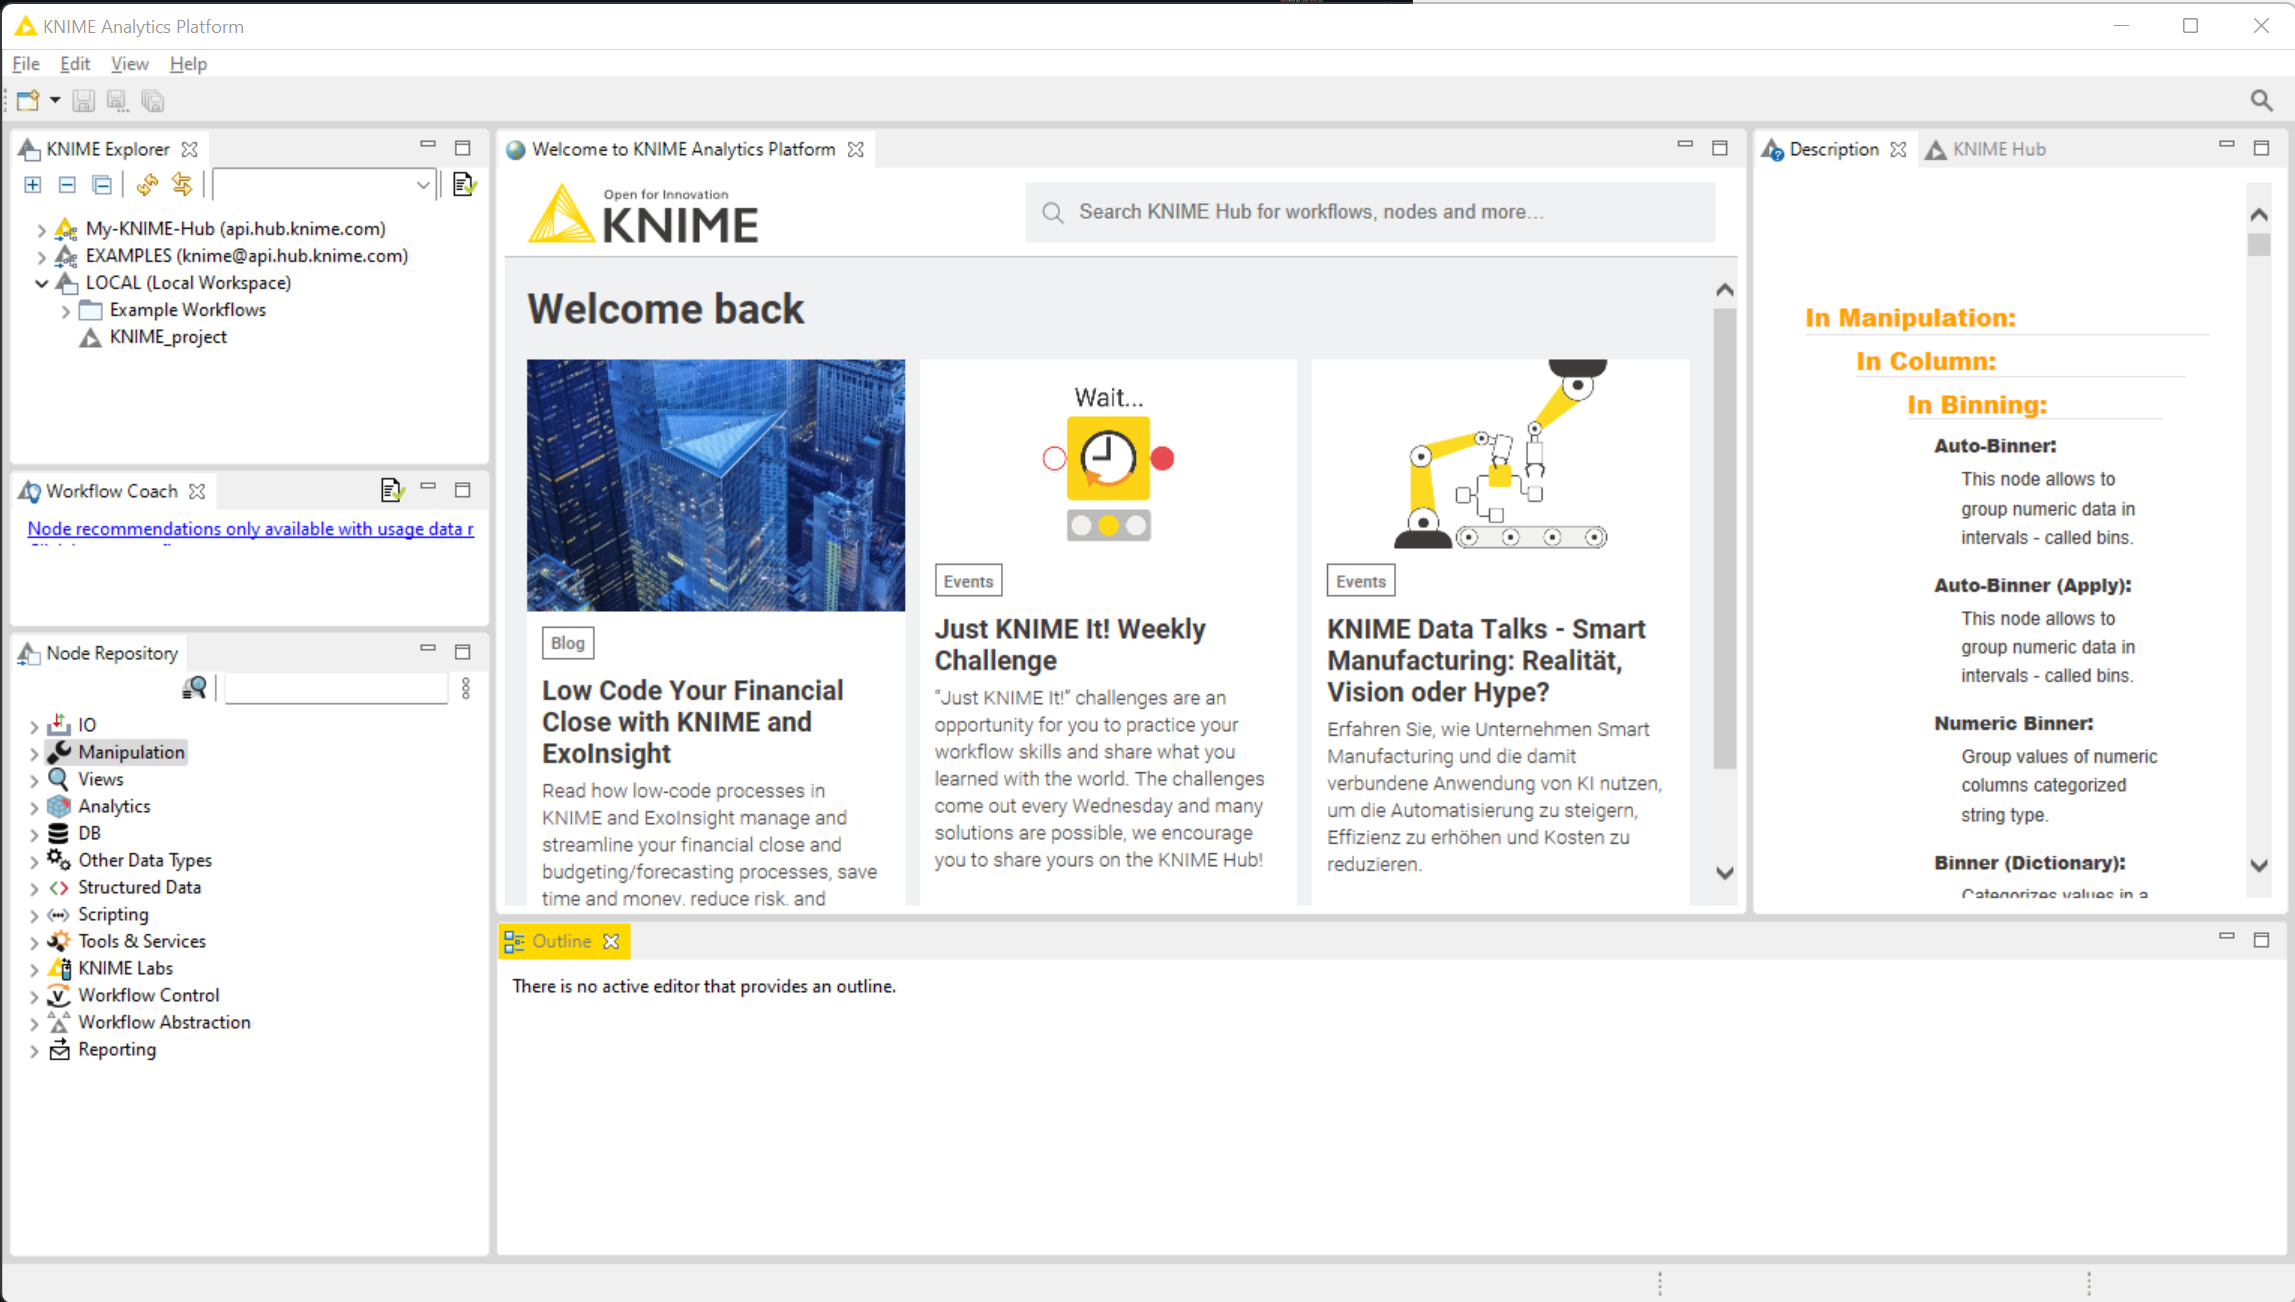
\includegraphics[width=.8\textwidth]{interfejs_programu.png}
    \label{fig:interfejs_programu}
    \caption{Interfejs zainstalowanego programu \enquote{Knime}}
\end{figure}

\zadanie{Utworzyć nowy projekt i wczytać dane z pliku \texttt{.csv}}

Tworzenie projektu (tzw. \enquote{workflow}) -- \ref{fig:tworzenie_nowego_projektu}.

\begin{figure}
    \centering
    \begin{subfigure}{.5\textwidth}
        \centering
        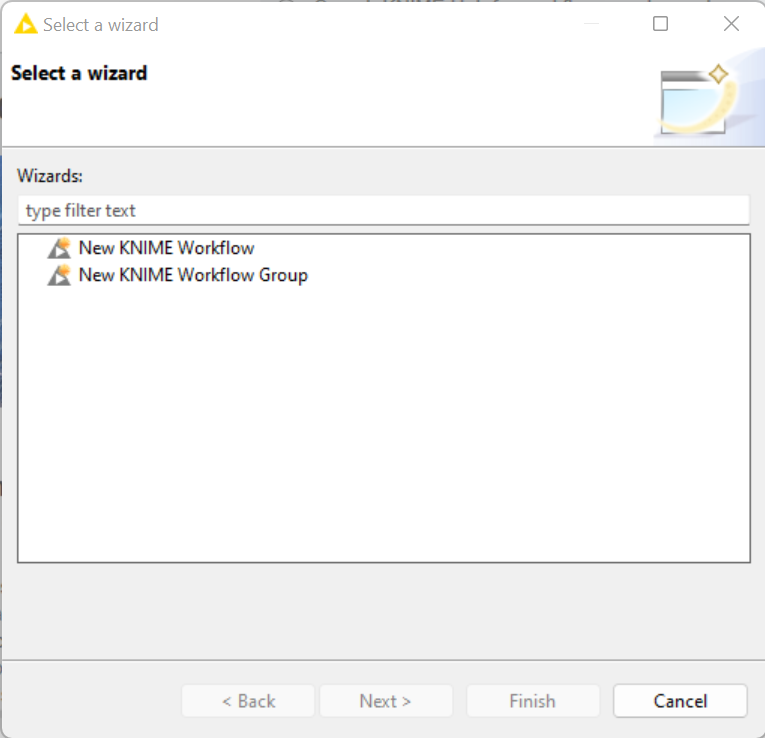
\includegraphics[width=.8\linewidth]{tworzenie_nowego_projektu.png}
        %   \caption{A subfigure}
        %   \label{fig:sub1}
    \end{subfigure}%
    \begin{subfigure}{.5\textwidth}
        \centering
        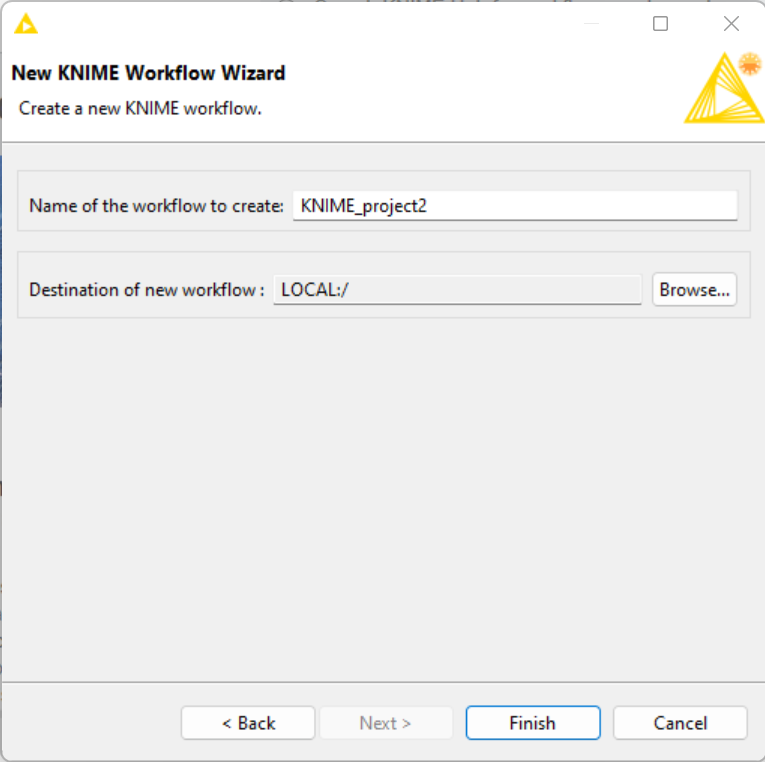
\includegraphics[width=.8\linewidth]{tworzenie_nowego_projektu_2.png}
        %   \caption{A subfigure}
        %   \label{fig:sub2}
    \end{subfigure}
    \caption{Tworzenie nowego projektu}
    \label{fig:tworzenie_nowego_projektu}
\end{figure}

Dodanie do przepływu (ang. \textit{workflow}) węzła \texttt{CSV Reader} pozwalającego wczytywać pliki \texttt{.csv} -- \ref{fig:csv_reader}.

\begin{figure}[h]
    \centering
    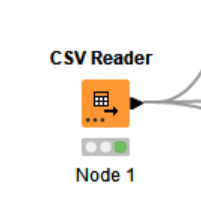
\includegraphics[width=.2\textwidth]{csv_reader.png}
    \caption{Węzeł wczytujący pliki \texttt{.csv}\label{fig:csv_reader}}
\end{figure}

Dostępne ustawienia deserializacji pliku \texttt{.csv} (rys. \ref{fig:csv_reader_2}):

\begin{itemize}
    \item separator wierszy (\textit{Row delimiter}),
    \item separator kolumn (\textit{Column delimiter}),
    \item ograniczniki napisów (\textit{Quote char}),
    \item automatyczne rozpoznawanie nagłówków (\textit{Has column header}).
\end{itemize}

\begin{figure}[h]
    \centering
    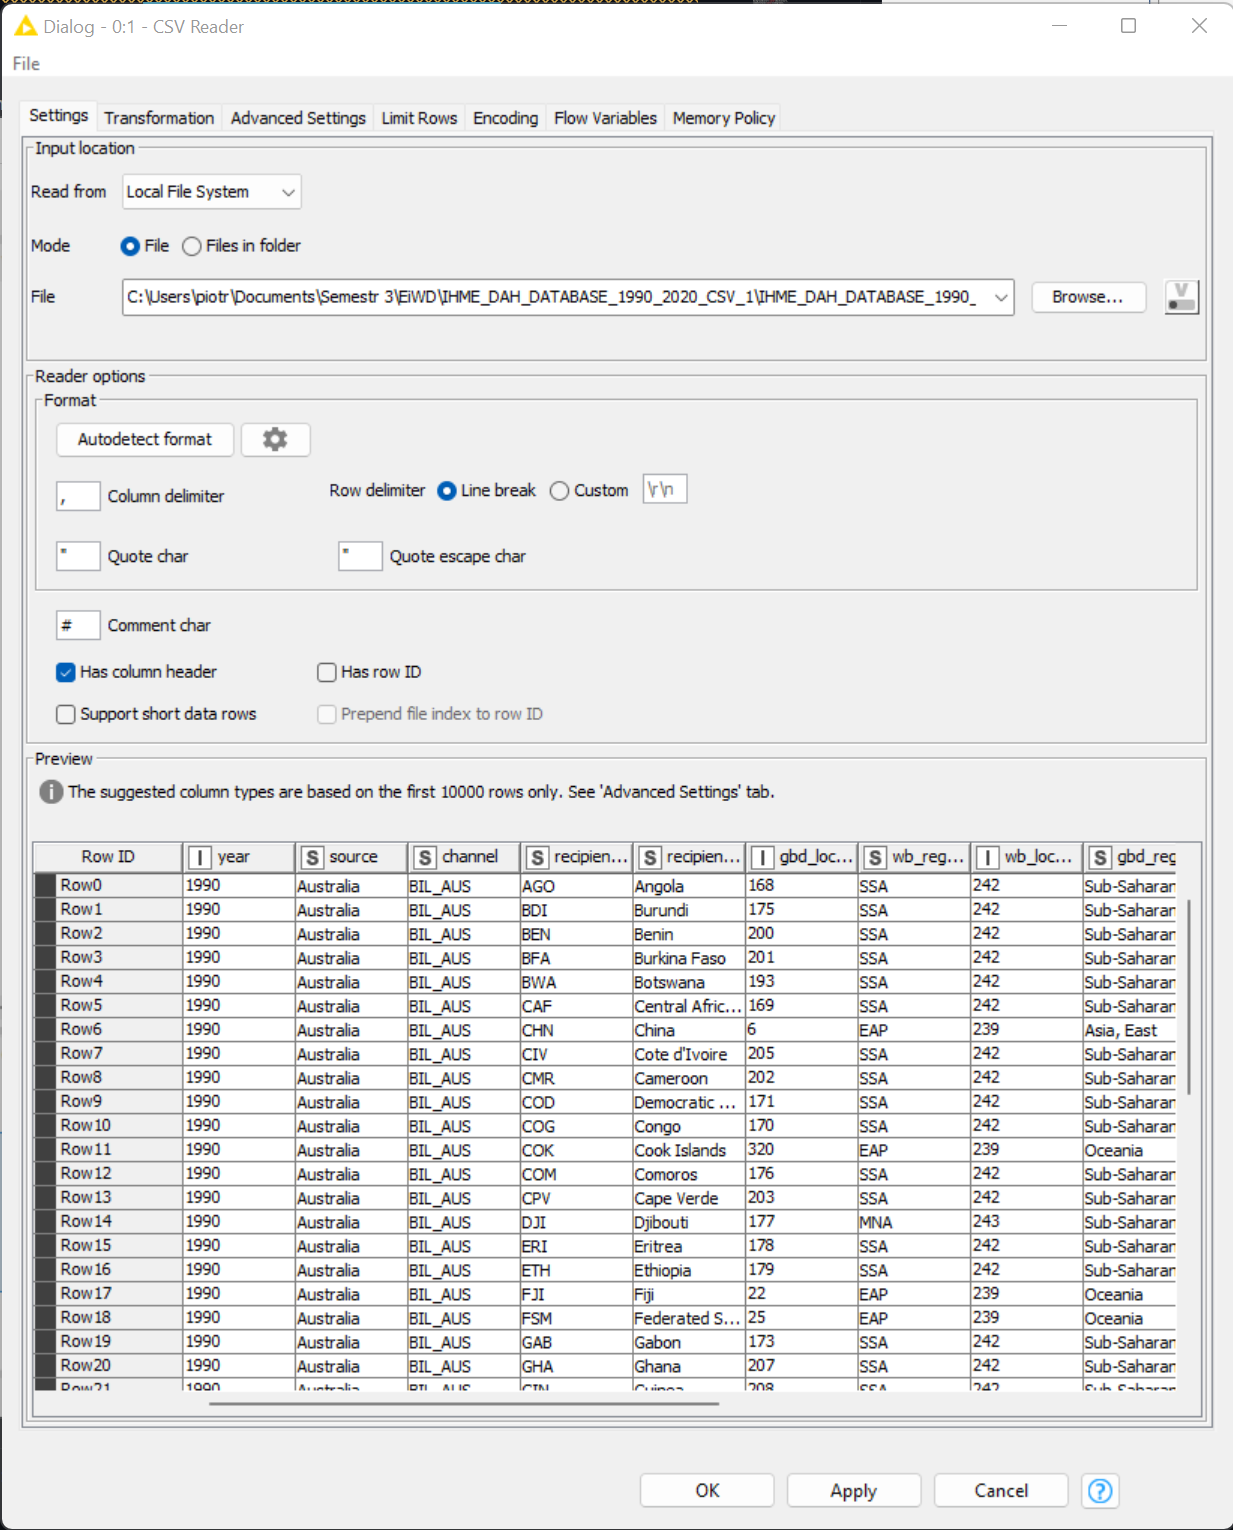
\includegraphics[width=.8\textwidth]{csv_reader_2.png}
    \caption{Parametry deserializacji pliku \texttt{.csv}\label{fig:csv_reader_2}}
\end{figure}

Wybór kolumn i ustawianie typów danych -- \ref{fig:csv_reader_3}.

\begin{figure}[h]
    \centering
    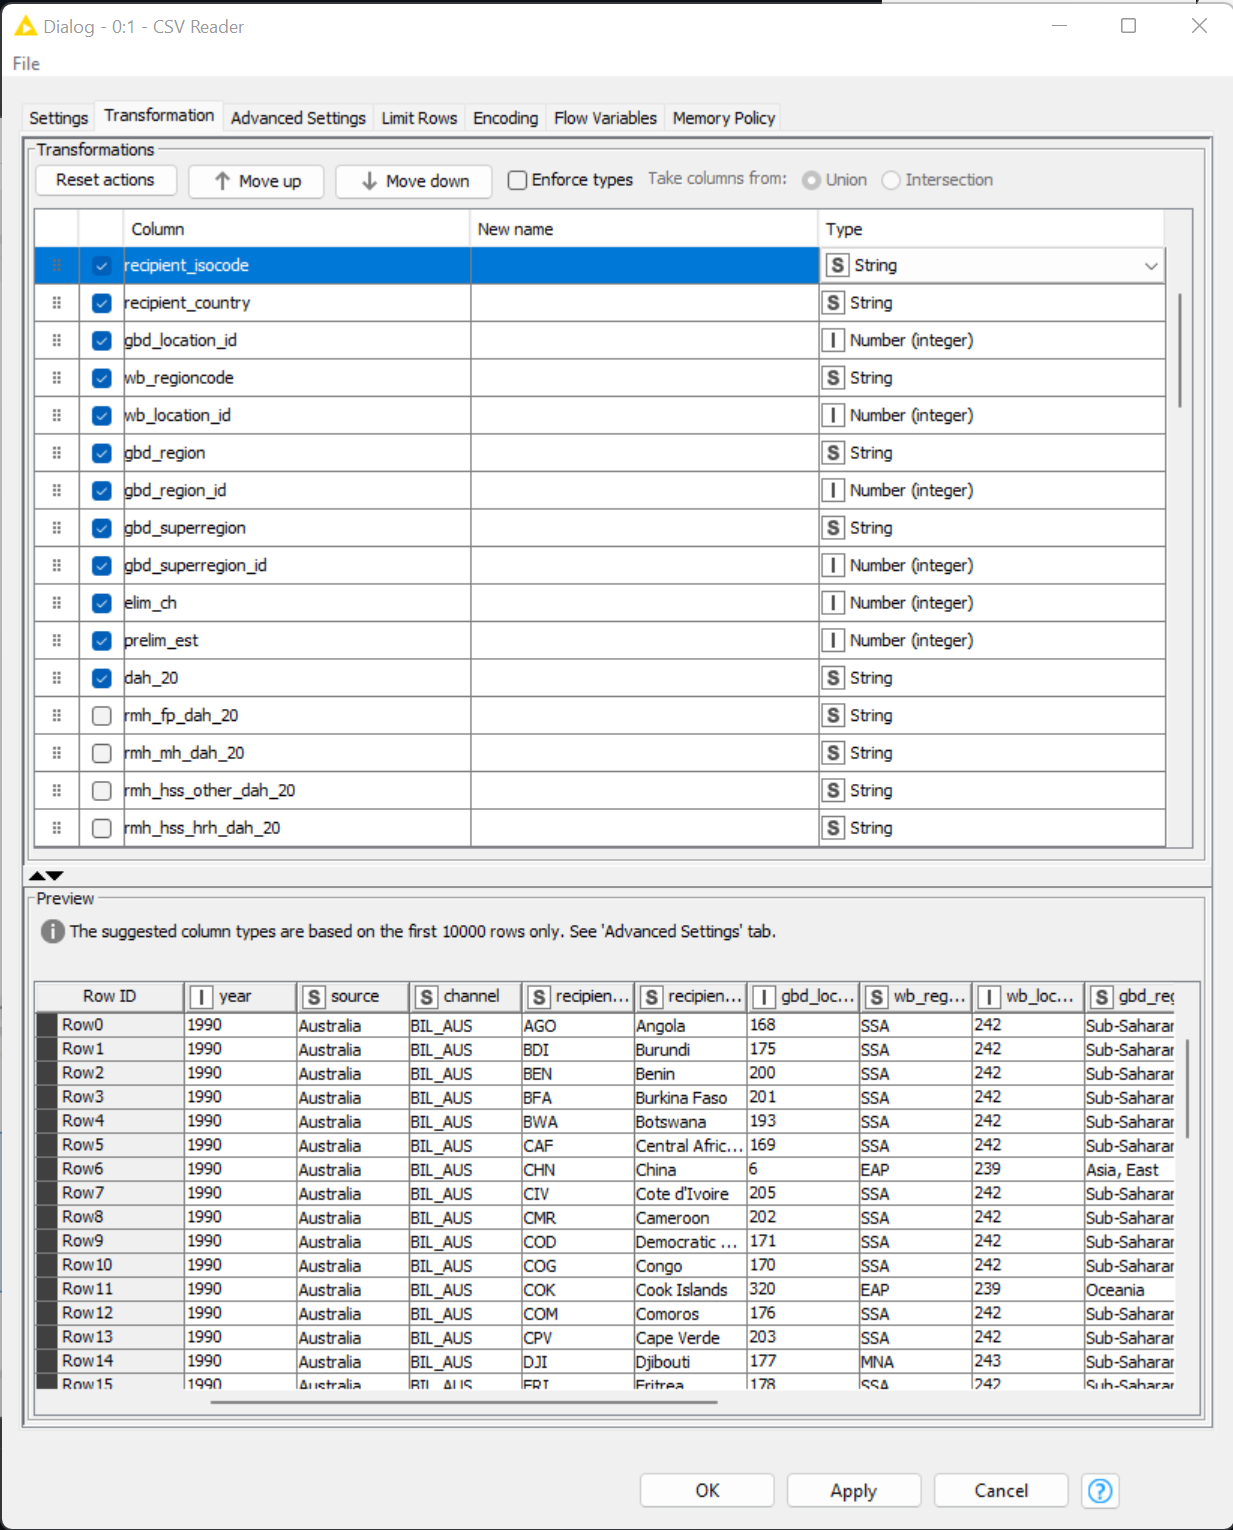
\includegraphics[width=.8\textwidth]{csv_reader_3.png}
    \caption{Okno wybierania kolumn i typu danych\label{fig:csv_reader_3}}
\end{figure}

Załadowanie danych przez wybranie komendy \enquote{Execute} -- \ref{fig:csv_reader_4}.

\begin{figure}[h]
    \centering
    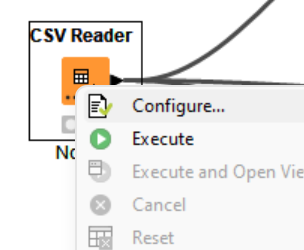
\includegraphics[width=.2\textwidth]{csv_reader_4.png}
    \caption{Uruchomienie węzła \texttt{CSV reader}\label{fig:csv_reader_4}}
\end{figure}

\zadanie{Wydzielić podgrupy danych numerycznych przy użyciu węzła \texttt{Numeric Binner}}

Dodanie do przepływu węzła \texttt{Numeric Binner} -- \ref{fig:numeric_binner}.

\begin{figure}[h]
    \centering
    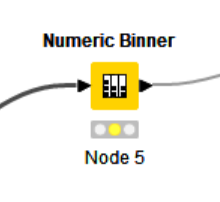
\includegraphics[width=.2\textwidth]{numeric_binner.png}
    \caption{Węzeł \texttt{Numeric Binner}\label{fig:numeric_binner}}
\end{figure}

Ustawienie przedziałów wartości na podstawie danych z kolumny \enquote{years}. Ustawione przedziały (rys. \ref{fig:numeric_binner_2}):

\begin{tabular}{lll}
    Nazwa          & Dolne ograniczenie & Górne ograniczenie \\ \hline
    Lata 1990-1992 & $-\inf$            & 1992               \\
    Lata 1992-1994 & 1992               & 1994               \\
    Lata 1994-1996 & 1994               & 1996               \\
    Lata 1996-1998 & 1996               & 1998               \\
    Lata 1998-     & 1998               & $\inf$             \\
\end{tabular}

\begin{figure}[h]
    \centering
    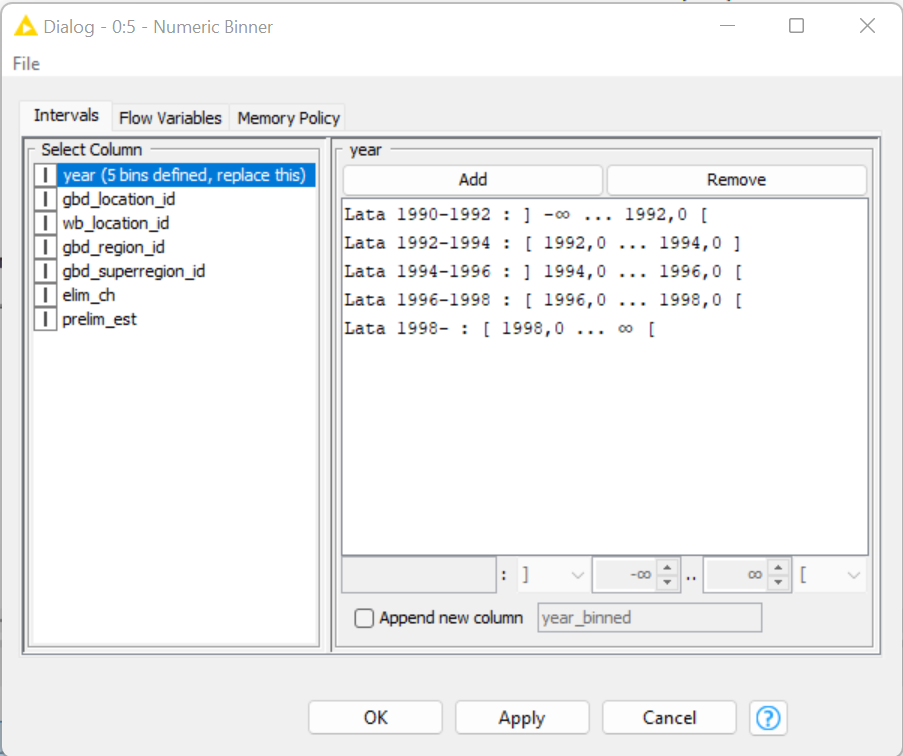
\includegraphics[width=.8\textwidth]{numeric_binner_2.png}
    \caption{Węzeł \texttt{Numeric Binner}\label{fig:numeric_binner_2}}
\end{figure}

Uruchomienie węzła -- analogicznie jak poprzednio (rys. \ref{fig:numeric_binner_3}).

\begin{figure}[h]
    \centering
    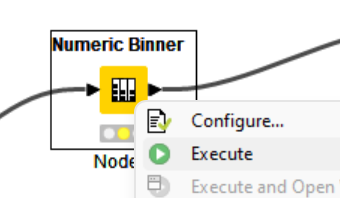
\includegraphics[width=.4\textwidth]{numeric_binner_3.png}
    \caption{Węzeł \texttt{Uruchomienie węzła \texttt{Numeric Binner}}\label{fig:numeric_binner_3}}
\end{figure}

\zadanie{Korzystając z danych podzielonych na podgrupy, wygenerować wykres rozrzutu}

Połączenie węzła \texttt{Scatter Plot} z uprzednio dodanymi do przepływu -- rys. \ref{fig:scatter_plot}.

\begin{figure}[h]
    \centering
    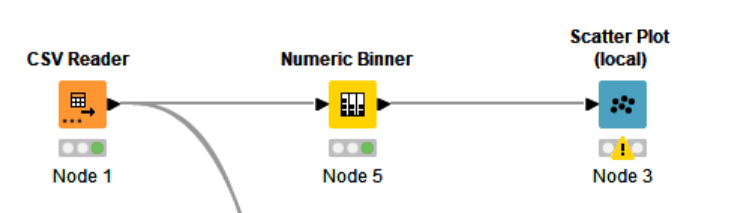
\includegraphics[width=.8\textwidth]{scatter_plot.png}
    \caption{Połączenie węzłów \texttt{CSV Reader}, \texttt{Numeric Binner}, \texttt{Scatter Plot}\label{fig:scatter_plot}}
\end{figure}

Ustawienia węzła \texttt{Scatter Plot}, generowanie i wyświetlanie wykresu -- rys. \ref{fig:scatter_plot_2}.

\begin{figure}
    \centering
    \begin{subfigure}{.3\textwidth}
        \centering
        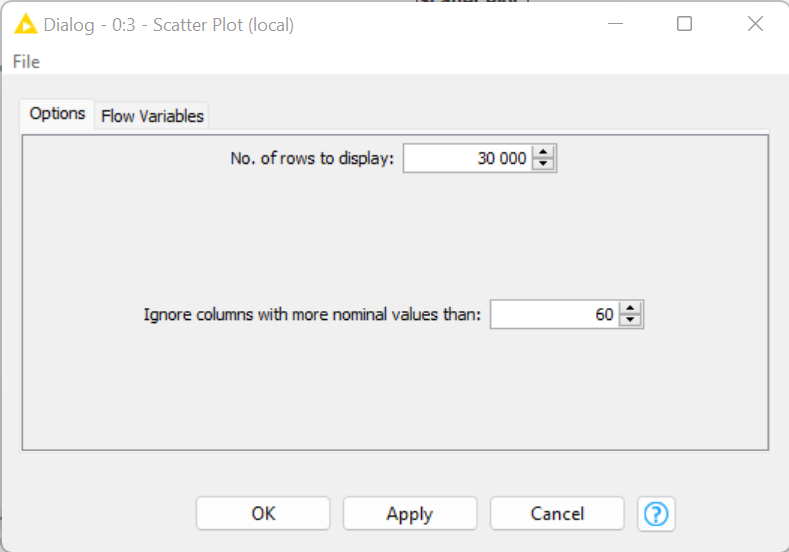
\includegraphics[width=0.9\linewidth]{scatter_plot_2.png}
        %   \caption{A subfigure}
        %   \label{fig:sub1}
    \end{subfigure}%
    \begin{subfigure}{.3\textwidth}
        \centering
        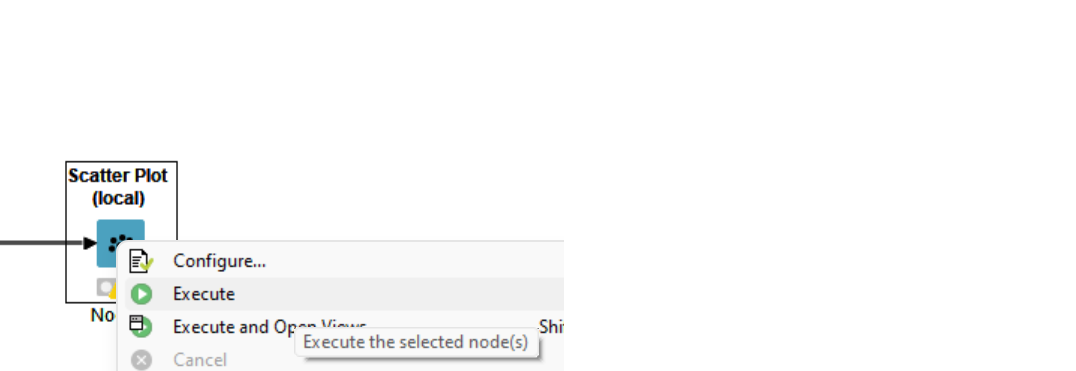
\includegraphics[width=1.0\linewidth]{scatter_plot_3.png}
        %   \caption{A subfigure}
        %   \label{fig:sub2}
    \end{subfigure}
    \begin{subfigure}{.3\textwidth}
        \centering
        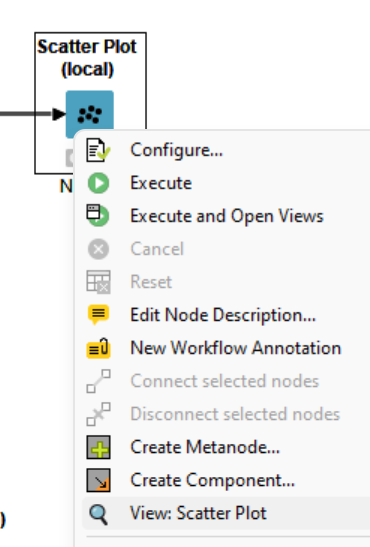
\includegraphics[width=.6\linewidth]{scatter_plot_4.png}
        %   \caption{A subfigure}
        %   \label{fig:sub2}
    \end{subfigure}
    \caption{Ustawienia węzła \texttt{Scatter Plot}, uruchomienie i wyświetlanie wykresu}
    \label{fig:scatter_plot_2}
\end{figure}

Uzyskany wykres -- rys. \ref{fig:scatter_plot_5}.

\begin{figure}[h]
    \centering
    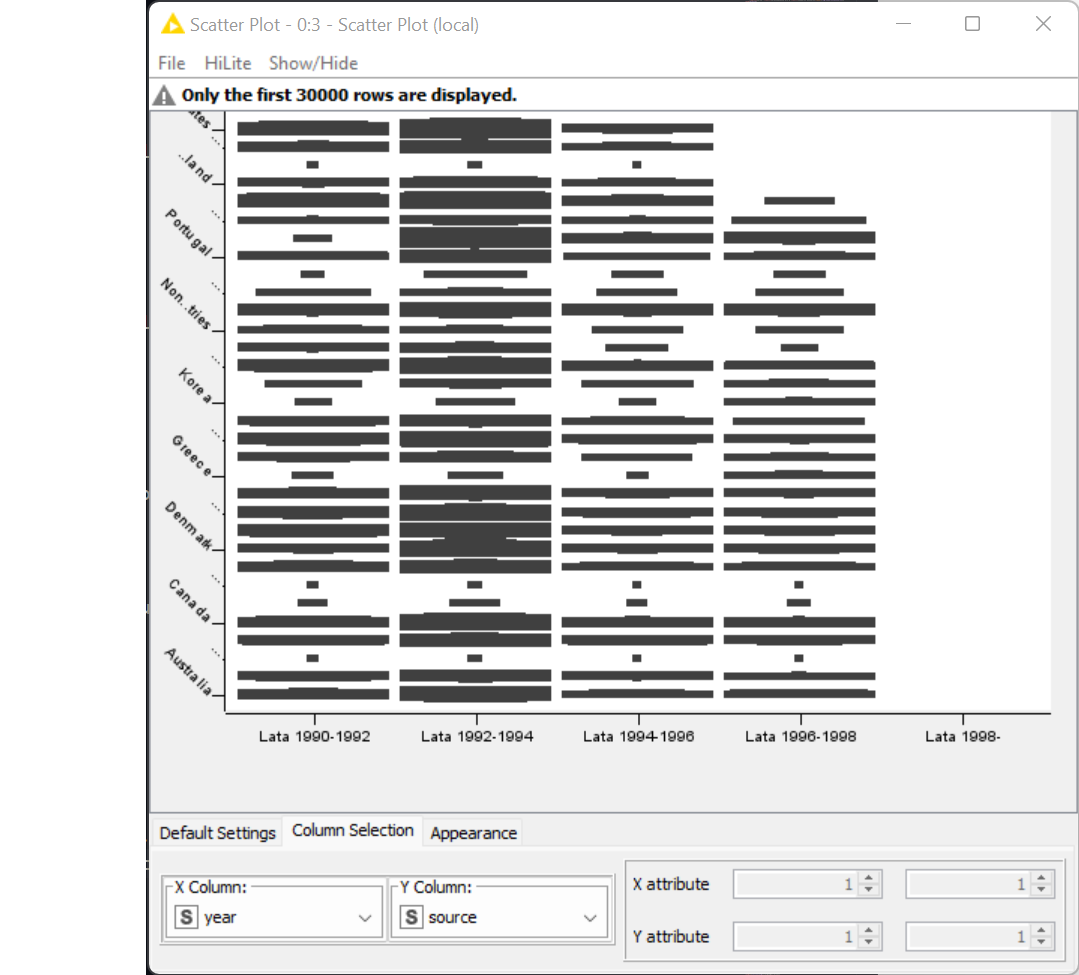
\includegraphics[width=.8\textwidth]{scatter_plot_5.png}
    \caption{Wykres rozrzutu na podstawie danych z kolumny \enquote{year} (podzielonych na 5 przedziałów) i \enquote{source}\label{fig:scatter_plot_5}}
\end{figure}

\zadanie{Wygenerować histogram}

Dodanie węzła generującego histogram do węzła \texttt{CSV Reader} i wskazanie, jakie dane zawierać będzie histogram (w przykładzie -- kolumny \enquote{year}, \enquote{gbd\_location\_id}, \enquote{gbd\_region\_id}).

\begin{figure}
    \centering
    \begin{subfigure}{.5\textwidth}
        \centering
        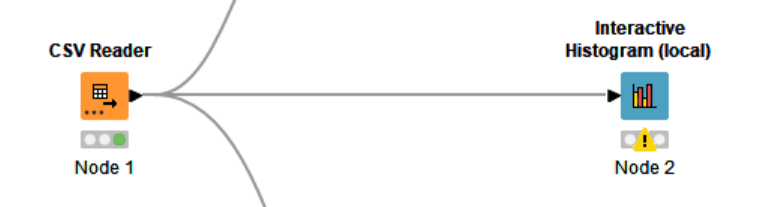
\includegraphics[width=.9\linewidth]{histogram.png}
        %   \caption{A subfigure}
        %   \label{fig:sub1}
    \end{subfigure}%
    \begin{subfigure}{.5\textwidth}
        \centering
        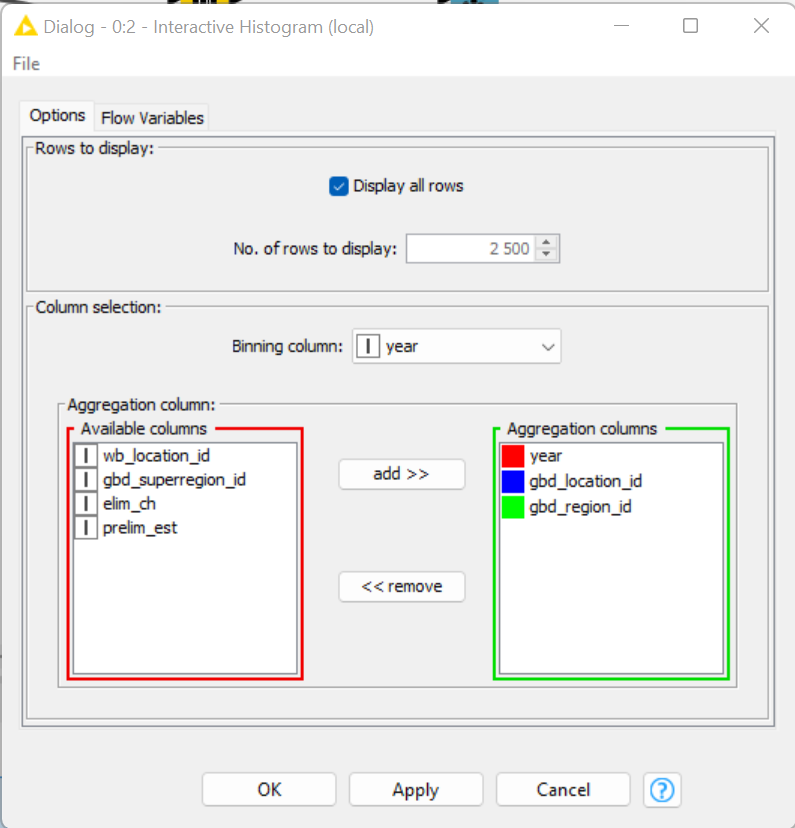
\includegraphics[width=.9\linewidth]{histogram_2.png}
        %   \caption{A subfigure}
        %   \label{fig:sub2}
    \end{subfigure}
    \caption{Węzeł histogramu i jego ustawienia}
    \label{fig:histogram}
\end{figure}

Wygenerowany histogram i dodatkowe ustawienia: \texttt{binning column} -- kolumna, względem której dzielone są wartości, \texttt{Aggregation method} -- zastosowana miara (w przykładzie -- \texttt{row count} -- liczba wierszy) -- rys. \ref{fig:histogram_3}

\begin{figure}[h]
    \centering
    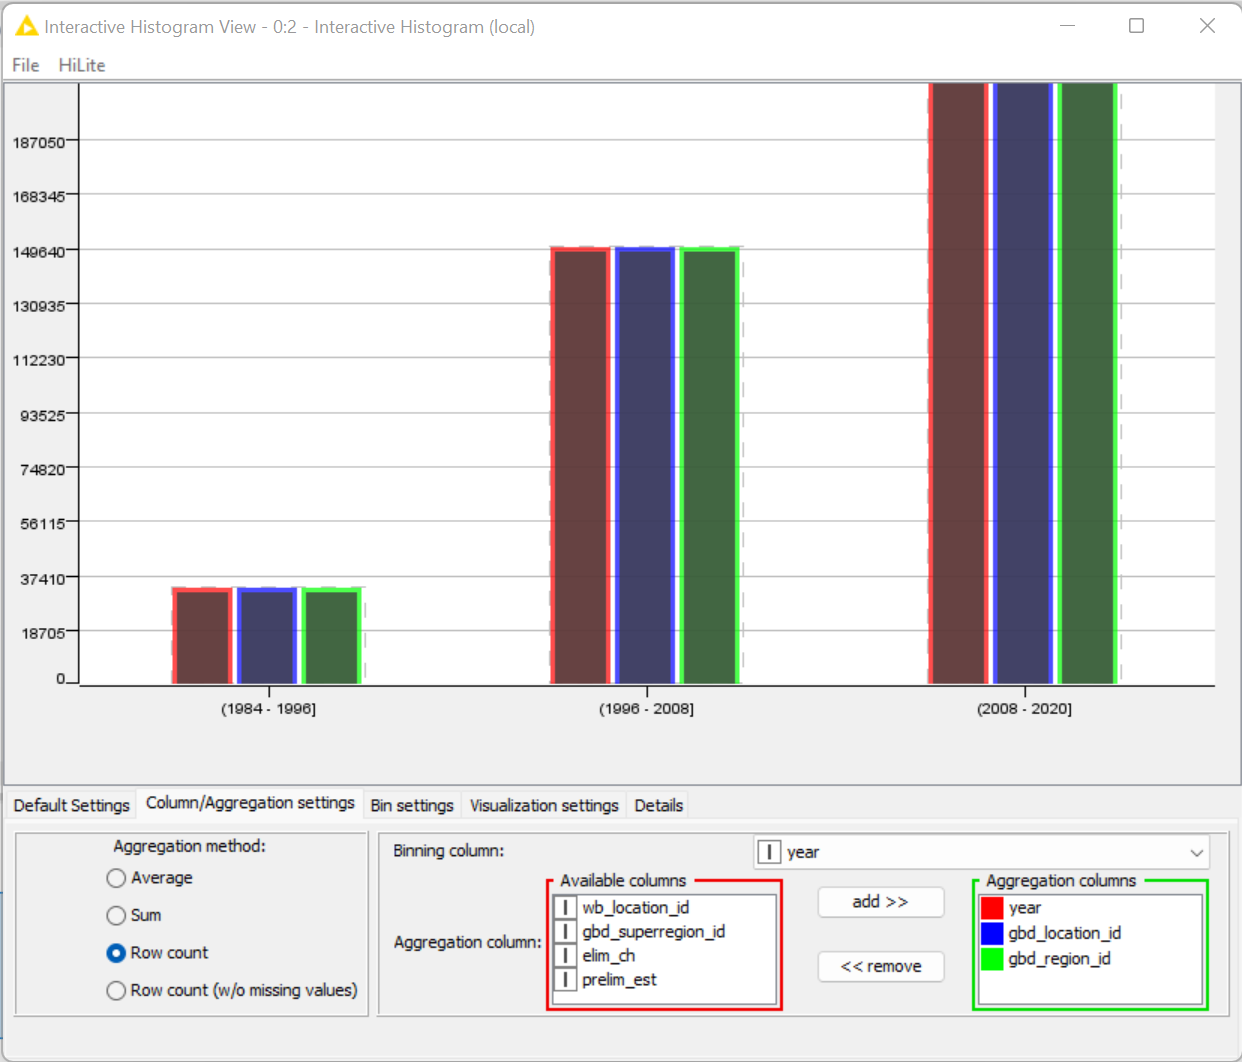
\includegraphics[width=.8\textwidth]{histogram_3.png}
    \caption{Wygenerowany histogram i dodatkowe ustawienia wykresu\label{fig:histogram_3}}
\end{figure}

\zadanie{Wygenerować macierz wykresów rozrzutu}

Węzeł generujący macierz wykresów rozrzutu podłączony do źródła danych -- \ref{fig:scatter_matrix}

\begin{figure}[h]
    \centering
    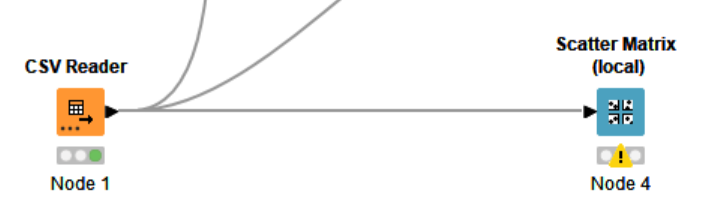
\includegraphics[width=.8\textwidth]{scatter_matrix.png}
    \caption{Połączenie węzłu \texttt{Scatter Matrix} ze źródłem danych (plik \texttt{.csv})\label{fig:scatter_matrix}}
\end{figure}

Wygenerowany wykres i jego ustawienia -- wybór danych do każdego wykresu w macierzy (w przykładzie kolumny \enquote{year}, \enquote{source}, \enquote{channel}) -- rys. \ref{fig:scatter_matrix_2}.

\begin{figure}[h]
    \centering
    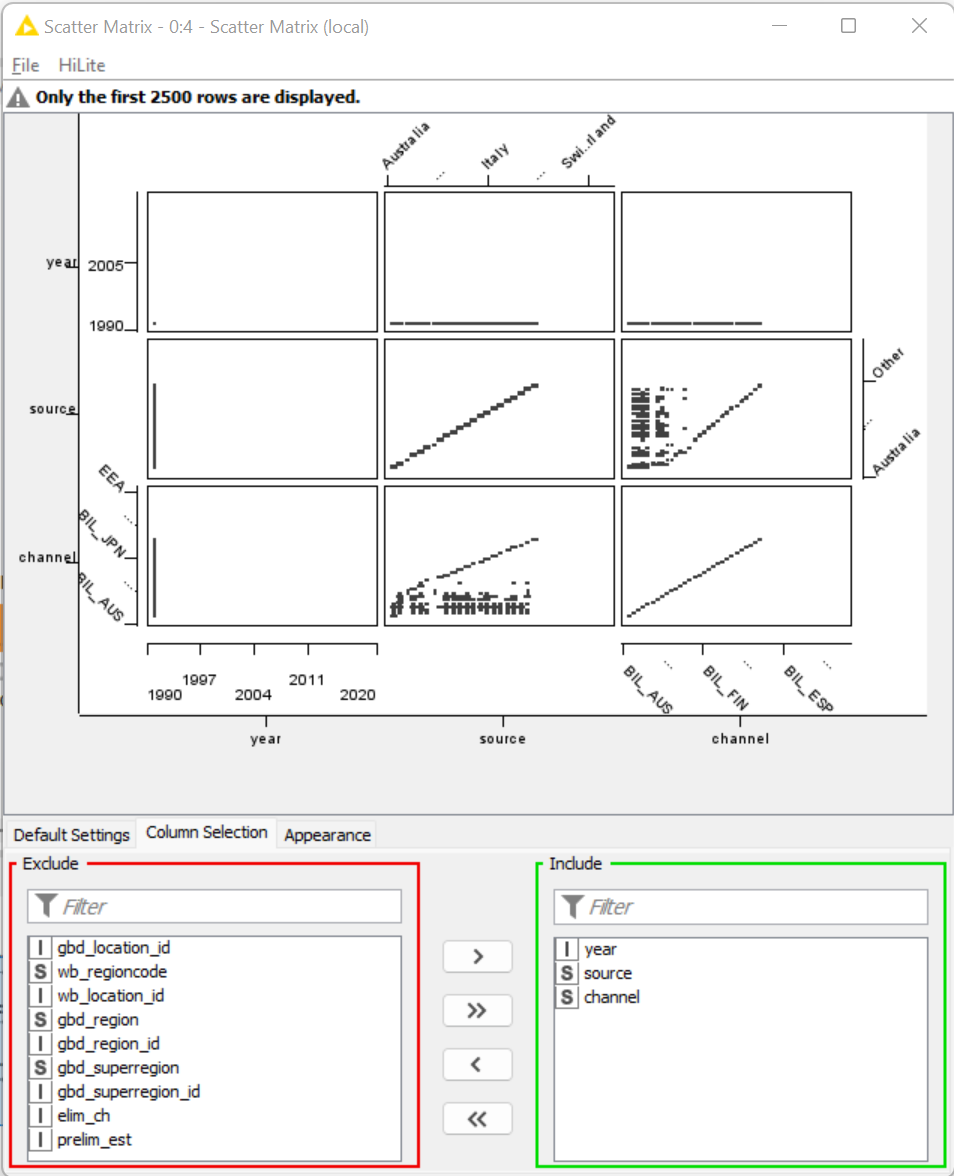
\includegraphics[width=.8\textwidth]{scatter_matrix_2.png}
    \caption{Wygenerowana macierz wykresów rozrzutu i jej ustawienai\label{fig:scatter_matrix_2}}
\end{figure}

\chapter*{Wnioski}

W programie \texttt{KNIME} przetwarzanie danych polega na ułożeniu odpowiednich węzłów (ang. \textit{nodes}) w tzw. przepływie -- rys. \ref{fig:przestrzen_pracy}.

\begin{figure}[h]
    \centering
    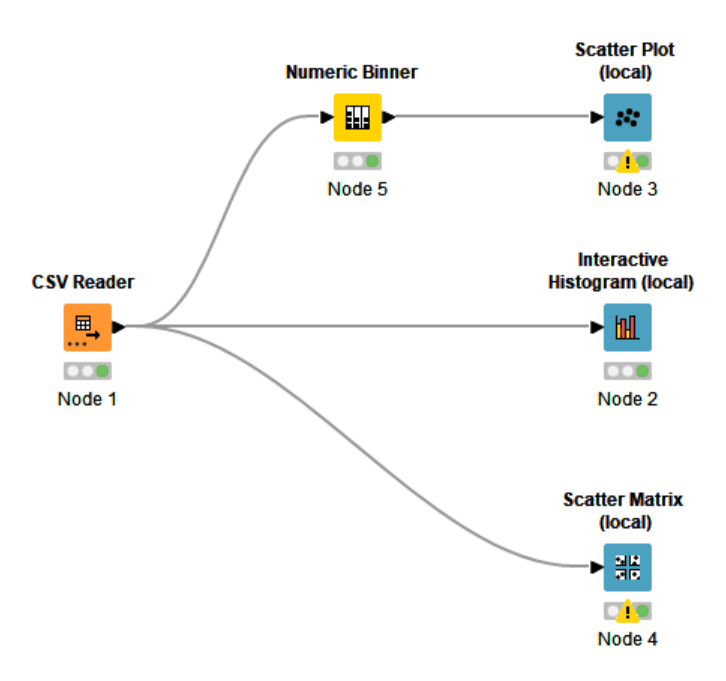
\includegraphics[width=.8\textwidth]{przestrzen_pracy.png}
    \caption{Układ węzłów w przepływie\label{fig:przestrzen_pracy}}
\end{figure}

Istnieje kilka rodzajów węzłów, m.in.

\begin{itemize}
    \item węzły pobierające dane, np. \texttt{CSV Reader} -- rys. \ref{fig:wezly_odczytujace};
    \item węzły przetwarzające dane, np. \texttt{Numeric Binner} -- rys. \ref{fig:wezly_przetwarzajace};
    \item węzły wizualizujące dane, np. \texttt{Scatter Plot} -- rys. \ref{fig:wezly_wizualizujace};
\end{itemize}

\begin{figure}[h]
    \centering
    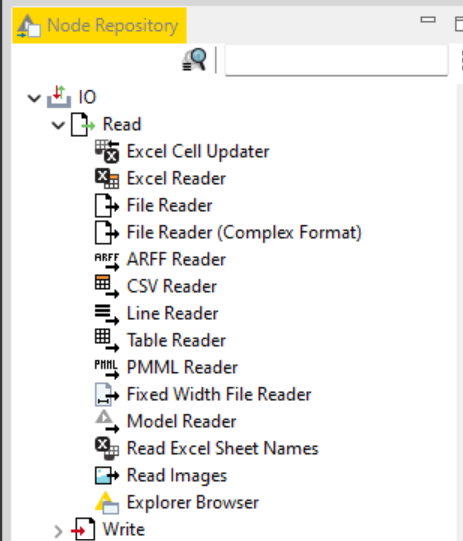
\includegraphics[width=.6\textwidth]{wezly_odczytujace.png}
    \caption{Węzły odczytujące dostępne w programie \texttt{KNIME}\label{fig:wezly_odczytujace}}
\end{figure}

\begin{figure}[h]
    \centering
    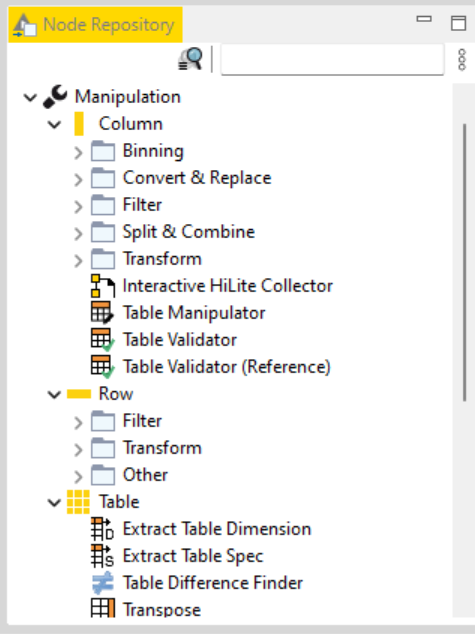
\includegraphics[width=.6\textwidth]{wezly_przetwarzajace.png}
    \caption{Węzły przetwarzające dane w programie \texttt{KNIME}\label{fig:wezly_przetwarzajace}}
\end{figure}

\begin{figure}[h]
    \centering
    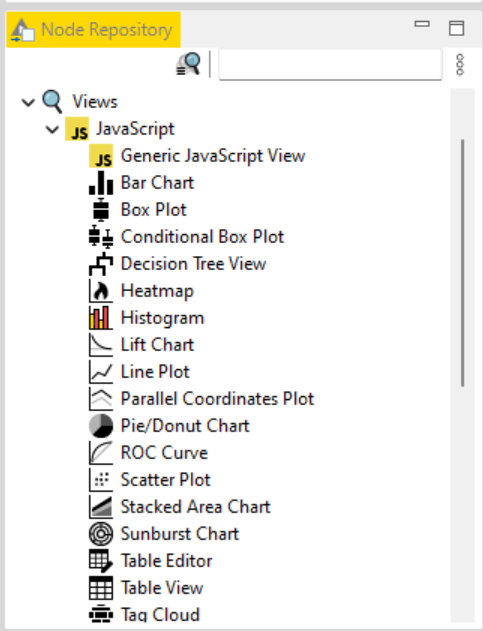
\includegraphics[width=.6\textwidth]{wezly_wizualizujace.png}
    \caption{Węzły wizualizujące dane w programie \texttt{KNIME}\label{fig:wezly_wizualizujace}}
\end{figure}

Podwójne kliknięcie w każdy węzeł prowadzi do jego ustawień. W przypadku węzłów wizualizujących najważniejsze ustawienia dostępne są po wyświetleniu danej wizualizacji.

Dane przechowywane w węźle nie są od razu dostępne po jego dodaniu do przepływu. Można je w każdej chwili usunąć opcją \texttt{Reset}. Wykorzystanie węzła lub węzłów pobierających z niego dane wymaga zawsze załadowania danych opcją \texttt{Execute}.

%\cleardoublepage

\printbibliography[heading=subbibliography,title={Strony internetowe},keyword=www]

\end{document}